\documentclass[border=10pt]{standalone}
\usepackage[T1]{fontenc}
\usepackage{tikz}
\usepackage[svgnames]{xcolor}
\usetikzlibrary{arrows.meta, positioning, calc, decorations.pathmorphing,
                 decorations.markings}

\colorlet{OrangeFill}{LightSalmon}
\colorlet{OrangeLine}{DarkSalmon!30!Chocolate}
\colorlet{GreenFill}{MediumAquamarine}
\colorlet{GreenLine}{MediumAquamarine!30!Teal}
\colorlet{PurpleFill}{MediumPurple}
\colorlet{PurpleLine}{MediumPurple!30!SlateBlue}
\colorlet{PinkFill}{Thistle}
\colorlet{PinkLine}{Thistle!30!Plum}
\colorlet{BlueFill}{LightSkyBlue}
\colorlet{BlueLine}{SteelBlue}
\colorlet{GrayFill}{LightGray!60!OldLace}
\colorlet{GrayLine}{RosyBrown!50!Silver}

\begin{document}
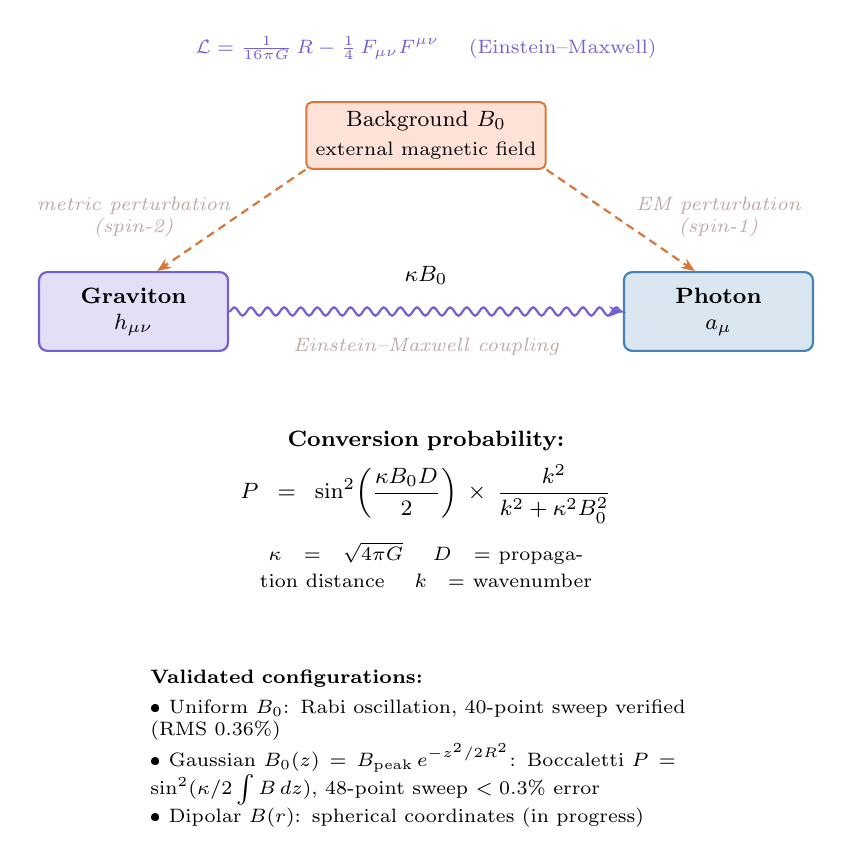
\begin{tikzpicture}[
    field/.style={
        rectangle, rounded corners=3pt, minimum width=2.4cm,
        minimum height=1.0cm, draw=#1, line width=0.8pt,
        fill=#1!20, font=\footnotesize\bfseries, align=center,
        text opacity=1, text=black
    },
    field/.default={black!70},
    bg/.style={
        rectangle, rounded corners=2pt, minimum width=2.0cm,
        minimum height=0.7cm, draw=OrangeLine, line width=0.7pt,
        fill=OrangeFill, fill opacity=0.3, font=\footnotesize,
        align=center, text opacity=1
    },
    annot/.style={font=\scriptsize\itshape, text=GrayLine, align=center},
    formula/.style={font=\footnotesize, align=center},
    arr/.style={-{Stealth[length=5pt, width=4pt]}, thick},
    wavy/.style={
        decorate, decoration={snake, amplitude=1.5pt, segment length=6pt},
        thick
    },
    node distance=1.0cm
]

% ===================================================================
% FIELDS
% ===================================================================

% Graviton
\node[field=PurpleLine] (grav) {Graviton\\$h_{\mu\nu}$};
\node[annot, above=0.3cm of grav] {metric perturbation\\(spin-2)};

% Photon
\node[field=BlueLine, right=5.0cm of grav] (phot) {Photon\\$a_\mu$};
\node[annot, above=0.3cm of phot] {EM perturbation\\(spin-1)};

% Background B-field (above, between)
\node[bg, above=1.8cm of $(grav)!0.5!(phot)$] (bfield)
    {Background $B_0$\\[1pt]\scriptsize external magnetic field};

% ===================================================================
% COUPLING ARROWS
% ===================================================================

% Bidirectional wavy coupling
\draw[wavy, PurpleLine, -{Stealth[length=5pt]}]
    (grav.east) -- (phot.west)
    node[midway, above=6pt, font=\footnotesize\bfseries, text=black]
    {$\kappa B_0$}
    node[midway, below=6pt, annot] {Einstein--Maxwell coupling};

% B-field influence
\draw[arr, OrangeLine, densely dashed]
    (bfield.south west) -- ($(grav.north)+(0.3,0)$);
\draw[arr, OrangeLine, densely dashed]
    (bfield.south east) -- ($(phot.north)+(-0.3,0)$);

% ===================================================================
% CONVERSION FORMULA
% ===================================================================
\node[formula, below=1.4cm of $(grav)!0.5!(phot)$,
      text width=7.0cm] (conv) {%
    \textbf{Conversion probability:}\\[4pt]
    $\displaystyle P = \sin^2\!\left(\frac{\kappa B_0 D}{2}\right)
    \times \frac{k^2}{k^2 + \kappa^2 B_0^2}$\\[6pt]
    \scriptsize $\kappa = \sqrt{4\pi G}$ \quad
    $D = $ propagation distance \quad
    $k = $ wavenumber};

% ===================================================================
% CONFIGURATIONS (below formula)
% ===================================================================
\node[below=0.8cm of conv, font=\scriptsize, align=left,
      text width=7.0cm] (configs) {%
    \textbf{Validated configurations:}\\[3pt]
    \textbullet\ Uniform $B_0$: Rabi oscillation, 40-point sweep verified
    (RMS 0.36\%)\\
    \textbullet\ Gaussian $B_0(z) = B_{\mathrm{peak}}\,e^{-z^2/2R^2}$:
    Boccaletti $P = \sin^2(\kappa/2 \int B\,dz)$,
    48-point sweep $< 0.3\%$ error\\
    \textbullet\ Dipolar $B(r)$: spherical coordinates (in progress)};

% ===================================================================
% LAGRANGIAN
% ===================================================================
\node[above=0.4cm of bfield, font=\scriptsize, align=center,
      text=PurpleLine] {%
    $\mathcal{L} = \frac{1}{16\pi G}\,R
    - \frac{1}{4}\,F_{\mu\nu}F^{\mu\nu}$
    \quad (Einstein--Maxwell)};

\end{tikzpicture}
\end{document}
